\documentclass{article}

\PassOptionsToPackage{numbers,sort&compress}{natbib}
\usepackage[preprint]{../../neurips}
\usepackage[utf8]{inputenc}
\usepackage[T1]{fontenc}
\usepackage{hyperref}
\usepackage{url}
\usepackage{booktabs}
\usepackage{amsfonts}
\usepackage{nicefrac}
\usepackage{microtype}
\usepackage{xcolor}
\usepackage{graphicx}
\usepackage{subcaption}
\usepackage{multirow}
\usepackage{array}
\usepackage{float}
\usepackage{adjustbox}
\usepackage{amsthm}
\usepackage{amsmath}
\usepackage{amssymb}
\usepackage{mathtools}
\usepackage{enumitem}
\usepackage{algorithm}
\usepackage{algpseudocode}
\usepackage{bm}

\graphicspath{{figures/}}

\title{Trajectory Spectral Filtering: Post-hoc Domain Generalization by Smoothing the Checkpoint Update Path}
\author{Anonymous Authors}

\newtheorem{theorem}{Theorem}
\newtheorem{proposition}{Proposition}
\newtheorem{lemma}{Lemma}
\newtheorem{corollary}{Corollary}
\newtheorem{definition}{Definition}
\newtheorem{assumption}{Assumption}
\newtheorem{remark}{Remark}

\newcommand{\RR}{\mathbb{R}}
\newcommand{\EE}{\mathbb{E}}
\newcommand{\PP}{\mathbb{P}}
\newcommand{\cB}{\mathcal{B}}
\newcommand{\cC}{\mathcal{C}}
\newcommand{\cG}{\mathcal{G}}
\newcommand{\cQ}{\mathcal{Q}}
\newcommand{\cR}{\mathcal{R}}
\newcommand{\cS}{\mathcal{S}}
\newcommand{\cU}{\mathcal{U}}
\newcommand{\cV}{\mathcal{V}}
\newcommand{\cZ}{\mathcal{Z}}
\newcommand{\argmin}{\operatorname*{arg\,min}}
\newcommand{\argmax}{\operatorname*{arg\,max}}
\newcommand{\diag}{\operatorname{diag}}
\newcommand{\Top}{\operatorname{Top}}
\newcommand{\CVaR}{\operatorname{CVaR}}
\newcommand{\tr}{\operatorname{tr}}
\newcommand{\rank}{\operatorname{rank}}
\newcommand{\simplex}{\Delta}
\newcommand{\iid}{i.i.d.}
\newcommand{\ood}{OOD}
\newcommand{\tsf}{\textup{\textsc{TSF}}}
\newcommand{\swad}{\textup{\textsc{SWAD}}}
\newcommand{\eoa}{\textup{\textsc{EoA}}}
\newcommand{\miro}{\textup{\textsc{MIRO}}}
\newcommand{\erm}{\textup{\textsc{ERM}}}
\newcommand{\ermpp}{\textup{\textsc{ERM++}}}
\newcommand{\norm}[1]{\left\lVert #1 \right\rVert}
\newcommand{\abs}[1]{\left\lvert #1 \right\rvert}
\newcommand{\paren}[1]{\left( #1 \right)}
\newcommand{\bracks}[1]{\left[ #1 \right]}
\newcommand{\braces}[1]{\left\{ #1 \right\}}
\newcommand{\inner}[2]{\left\langle #1, #2 \right\rangle}
\newcommand{\loss}{\ell}
\newcommand{\TBD}{\textbf{TBD}}

\begin{document}

\maketitle

\begin{abstract}
Single-run post-hoc domain generalization matters because it can be attached to a strong empirical-risk-minimization pipeline without retraining and without test-time ensembles. Existing post-hoc methods in this regime mostly choose a checkpoint, average a window, or average a selected subset of checkpoints. This paper studies a different operator on the same trajectory object. We propose \textbf{\tsf{}} (\textbf{T}rajectory \textbf{S}pectral \textbf{F}iltering), a method that transforms the checkpoint-to-checkpoint update sequence of each parameter group along the checkpoint axis, shrinks high-temporal-frequency components, and reconstructs one final model from the filtered update path. The main filter family is not heuristic: it is derived as the unique minimizer of a spectral Sobolev-type smoothing objective on the observed update sequence. We prove an exact variational characterization, derive the induced checkpoint coefficients of the final model, show that ordinary checkpoint averaging is a triangular update kernel inside the same update-space representation, prove nonexpansiveness of the filter, give an exact spectral bias--variance decomposition, establish a strict-improvement result for sufficiently small positive shrinkage under nontrivial penalized noise, derive a Sobolev-type error bound and a recovery theorem under vanishing additive noise, and connect parameter-space denoising to worst-case hidden-shift risk through a capped-simplex top-\(\alpha\) / empirical-\(\CVaR\) characterization and a uniform local smoothness bound. The experimental section is complete in protocol and published benchmark context, but every new \tsf{} result is intentionally left as \TBD{} because the method has not yet been run. The paper therefore makes a theory-and-method contribution first, while being explicit about what remains empirical.
\end{abstract}

\section{Introduction}

Single-run post-hoc model selection has become one of the most practical routes to domain generalization (DG). One trains a standard source-pooled model, saves dense checkpoints, and then chooses a single deployable predictor after training has already finished. The attraction is operational rather than philosophical: this regime works with standard code, standard backbones, and existing training budgets.

That practical attraction has already translated into strong published results. On the standard five-dataset DomainBed ResNet-50 suite, \swad{} improves the average accuracy of \erm{} from \(63.3\) to \(66.9\) across PACS, VLCS, OfficeHome, TerraIncognita, and DomainNet \citep{cha2021swad}. A stronger hybrid configuration that combines \miro{} with the same post-hoc selector reaches \(68.1\) in later published benchmark comparisons \citep{teterwak2025ermpp}. The broader weight-averaging literature further reinforces the message that the last checkpoint is often not the right deployment object: stochastic weight averaging \citep{izmailov2018swa}, fast geometric ensembling \citep{garipov2018fge}, model soups \citep{wortsman2022soups}, and weight EMA \citep{moralesbrotons2024ema} all exploit information distributed across a trajectory rather than trusting one endpoint.

Still, there is a recurring structural pattern. Current post-hoc DG methods mostly answer one of these questions:
\begin{itemize}[leftmargin=1.4em]
    \item Which checkpoint should be selected?
    \item Which contiguous window should be averaged?
    \item Which subset of checkpoints should be averaged?
\end{itemize}
These are reasonable questions, but they all operate by \emph{choosing points on the trajectory} and then aggregating them directly.

This paper studies a different question:
\begin{quote}
\textbf{Instead of choosing which checkpoints to average, can we filter the checkpoint update path itself and reconstruct a single model from the filtered dynamics?}
\end{quote}

The resulting method is \textbf{\tsf{}} (\textbf{T}rajectory \textbf{S}pectral \textbf{F}iltering). Let a training run produce checkpoints \(\theta^{(1)},\ldots,\theta^{(N)}\). For each architecture-aligned parameter group \(g\), form the checkpoint-to-checkpoint update sequence
\[
v_g^{(t)} = w_g^{(t+1)} - w_g^{(t)}, \qquad t=1,\ldots,N-1.
\]
\tsf{} applies an orthonormal transform along the checkpoint axis, shrinks high-temporal-frequency components by a derived spectral filter, inverts the transform, and reconstructs the final model from the filtered update path.

Two points are important.

First, \tsf{} is \emph{not} just ``frequency language'' pasted onto an arbitrary heuristic. The main filter family is derived exactly as the unique minimizer of a convex smoothing objective in spectral coordinates.

Second, \tsf{} does \emph{not} assume that checkpoint-time frequency has universal semantic meaning. The correct claim is narrower: if the observed update path contains a smooth component plus oscillatory contamination, then spectral filtering can recover a better update path than the raw endpoint. Whether that translates into better \ood{} generalization is then a separate question, and this paper treats it that way.

The paper makes six contributions.
\begin{enumerate}[leftmargin=1.4em]
    \item We formulate \tsf{}, a single-model post-hoc DG method that acts on groupwise checkpoint-to-checkpoint updates rather than selecting or averaging checkpoints directly.
    \item We derive the main \tsf{} filter family as the unique minimizer of a spectral Sobolev-type smoothing problem over the observed update sequence.
    \item We show exactly how \tsf{} induces checkpoint coefficients at the final endpoint, and prove that ordinary checkpoint averaging corresponds to a triangular update kernel in the same update-space representation.
    \item We give rigorous denoising guarantees: nonexpansiveness, exact bias--variance decomposition, strict improvement for sufficiently small positive shrinkage under nontrivial penalized noise, a Sobolev-type error bound, and a recovery theorem under vanishing additive noise.
    \item We connect \tsf{} to DG through a hidden-shift evaluation functional: a capped-simplex adversary equals top-\(\alpha\) empirical tail risk, and local uniform smoothness converts parameter error into worst-case hidden-shift loss error.
    \item We provide a complete experimental protocol, original figures, and exact published benchmark context from prior work, while leaving every new \tsf{} result as \TBD{}.
\end{enumerate}

\begin{figure}[t]
    \centering
    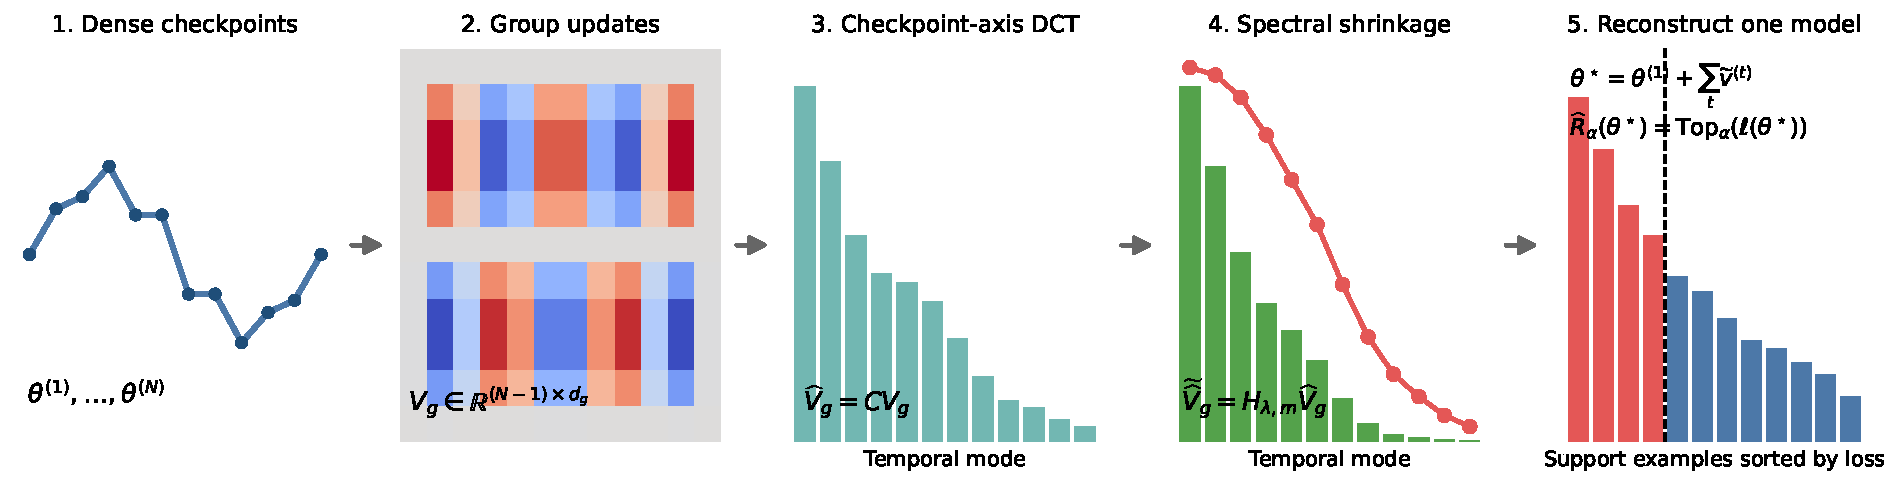
\includegraphics[width=\linewidth]{overview_pipeline.pdf}
    \caption{\textbf{\tsf{} overview.} A dense checkpoint trajectory is converted into groupwise update matrices. Each update sequence is transformed along the checkpoint axis, spectrally shrunk, inverted, and cumulatively reconstructed into one final model. The same model is then evaluated under hidden-shift tail risk on a pooled source holdout set.}
    \label{fig:overview}
\end{figure}

\section{Related Work}

\paragraph{Post-hoc domain generalization.}
\swad{} is the canonical single-run post-hoc DG reference: it uses dense late-trajectory averaging guided by a validation-based windowing rule and shows that flatter solutions can generalize better under shift \citep{cha2021swad}. \eoa{} studies moving averages within a run and heavier ensembles of averages across runs, explicitly positioning averaging as a better model-selection primitive for DG \citep{arpit2022eoa}. \miro{} improves the representation during training and then benefits again from the same post-hoc selector \citep{cha2022miro}. \tsf{} stays in this post-hoc regime, but changes the operator applied to the trajectory.

\paragraph{Weight averaging and trajectory geometry.}
SWA, FGE, linear mode connectivity, model soups, and weight-space interpolation methods such as WiSE-FT show that dense trajectories and nearby fine-tuned models often lie in connected low-loss regions where averaging is safe and useful \citep{izmailov2018swa,garipov2018fge,frankle2020linear,wortsman2022soups,wortsman2022wiseft}. Weight EMA adds another strong trajectory smoother and improves robustness and calibration in modern deep networks \citep{moralesbrotons2024ema}. \tsf{} is adjacent to this literature, but it does not average checkpoints directly; it smooths the update path in a transformed checkpoint-time coordinate system.

\paragraph{Trajectory information as signal.}
Recent work shows that learning trajectories themselves contain information about generalization \citep{fu2023trajectory}. This is important motivation for \tsf{}, but not a proof of it. Our method makes a more specific claim: groupwise checkpoint-to-checkpoint updates may admit a useful low-frequency / high-frequency decomposition along the checkpoint axis.

\paragraph{Memorization and training dynamics.}
The idea that deep networks learn simple/shared structure before idiosyncratic fitting is supported by memorization and spectral-bias studies \citep{arpit2017memorization,rahaman2019spectralbias}. At the same time, the training-dynamics view of spurious features warns that harmful features need not be exclusively late or high-frequency \citep{murali2023spurious}. We therefore use this literature as motivation and counter-motivation, not as a direct theorem source.

\paragraph{Risk under hidden subgroup shift.}
Worst-case subpopulation evaluation and minimax-regret learning provide a principled way to talk about distribution shift without assuming observed group labels \citep{li2021worstcase,agarwal2022mro}. \tsf{} uses this perspective only for evaluation and local theory: it does not optimize a subgroup-specific objective, but it can be analyzed under one.

\paragraph{Spectral editing of weights.}
Recent preprints explore spectral editing of single weight updates for robustness or ID/\ood{} trade-offs \citep{abdollahpoorrostam2026monosoup}. \tsf{} differs in the axis it spectralizes: the object here is the \emph{sequence of checkpoint-to-checkpoint updates}, not the singular directions inside one endpoint update.

\section{Problem Setup}
\label{sec:setup}

We work in the standard single-run post-hoc DG setting. A base learner produces dense checkpoints
\[
\theta^{(1)}, \theta^{(2)}, \ldots, \theta^{(N)} \in \RR^d.
\]
The post-hoc method is allowed to access:
\begin{itemize}[leftmargin=1.4em]
    \item the saved checkpoints,
    \item a pooled labeled source validation split \(\cV\), used only for reporting and optional hyperparameter tuning without source-domain labels,
    \item a pooled labeled source support split \(\cU=\braces{(x_i,y_i)}_{i=1}^n\), used only to define the hidden-shift evaluation functional.
\end{itemize}

Let \(\cG\) denote a partition of the model parameters into architecture-aligned groups, such as convolutional channels, attention heads, full projection matrices, or full tensor blocks. For group \(g\in\cG\), let
\[
w_g^{(t)} \in \RR^{d_g}
\]
be the flattened group parameters at checkpoint \(t\), so that \(\sum_{g\in\cG} d_g = d\).

\begin{definition}[Groupwise update sequence]
For each group \(g\), define the checkpoint-to-checkpoint update sequence
\[
v_g^{(t)} = w_g^{(t+1)} - w_g^{(t)}, \qquad t=1,\ldots,n_u,
\]
where \(n_u = N-1\). Stack the updates row-wise into
\[
V_g = 
\begin{bmatrix}
(v_g^{(1)})^\top \\
\vdots \\
(v_g^{(n_u)})^\top
\end{bmatrix}
\in \RR^{n_u \times d_g}.
\]
\end{definition}

The choice to operate on updates rather than absolute checkpoints is deliberate. Absolute trajectories are dominated by global drift. Update sequences make temporal roughness explicit while still allowing exact reconstruction of the endpoint.

\section{Trajectory Spectral Filtering}
\label{sec:method}

\subsection{A concrete filter family}

Let \(n=n_u\). Define the orthonormal DCT-II matrix \(C_n \in \RR^{n\times n}\) by
\begin{equation}
(C_n)_{jk} =
\begin{cases}
\sqrt{\frac{1}{n}}, & j=1, \\
\sqrt{\frac{2}{n}} \cos\!\left( \frac{\pi (j-1)(k-\tfrac12)}{n} \right), & 2\le j\le n,
\end{cases}
\qquad 1\le k\le n.
\label{eq:dct}
\end{equation}
For smoothing order \(m\in\mathbb{N}\), define
\begin{equation}
\omega_j = 2 \sin\!\left( \frac{\pi (j-1)}{2n} \right),
\qquad
\rho_j = \omega_j^{2m},
\qquad
\Lambda_m = \diag(\rho_1,\ldots,\rho_n).
\label{eq:freqs}
\end{equation}
The spectral shrinkage matrix is
\begin{equation}
H_{\lambda,m}
=
\diag\!\left( \frac{1}{1+\lambda \rho_1}, \ldots, \frac{1}{1+\lambda \rho_n} \right),
\qquad \lambda \ge 0.
\label{eq:filter}
\end{equation}

\begin{definition}[\tsf{} operator]
For group \(g\), the filtered update matrix is
\begin{equation}
\widetilde V_g(\lambda,m)
=
C_n^\top H_{\lambda,m} C_n V_g.
\label{eq:tsf_updates}
\end{equation}
Writing the rows of \(\widetilde V_g\) as \(\widetilde v_g^{(1)},\ldots,\widetilde v_g^{(n)}\), the filtered endpoint is
\begin{equation}
w_g^\star(\lambda,m)
=
w_g^{(1)} + \sum_{t=1}^{n} \widetilde v_g^{(t)}.
\label{eq:tsf_endpoint}
\end{equation}
The final filtered model is
\begin{equation}
\theta^\star(\lambda,m) = \braces{w_g^\star(\lambda,m) : g\in\cG }.
\label{eq:tsf_model}
\end{equation}
\end{definition}

\subsection{Why these terms appear}

The specific form in Eqs.~\eqref{eq:freqs}--\eqref{eq:filter} is not arbitrary. It is the closed-form solution of a spectral smoothing problem.

\begin{proposition}[Variational characterization]
\label{prop:variational}
Fix \(g\in\cG\), \(\lambda\ge 0\), and \(m\in\mathbb{N}\). Then \(\widetilde V_g(\lambda,m)\) is the unique minimizer of
\begin{equation}
\min_{U\in\RR^{n\times d_g}}
\;
\frac12 \norm{U - V_g}_F^2
+
\frac{\lambda}{2}
\norm{\Lambda_m^{1/2} C_n U}_F^2.
\label{eq:variational}
\end{equation}
Equivalently, \(\widetilde V_g\) is the unique minimizer of
\begin{equation}
\min_{U\in\RR^{n\times d_g}}
\;
\frac12 \norm{U - V_g}_F^2
+
\frac{\lambda}{2}
\inner{U}{Q_m U}_F,
\qquad
Q_m = C_n^\top \Lambda_m C_n.
\label{eq:variational_q}
\end{equation}
\end{proposition}

Proposition~\ref{prop:variational} is the main derivation result: \(\lambda\) is the roughness penalty weight and \(\rho_j\) is the frequency-dependent penalty applied in DCT coordinates. Higher temporal frequencies are penalized more heavily because \(\rho_j\) grows with \(j\).

\subsection{How \tsf{} differs from checkpoint averaging}

\tsf{} acts on updates, but the final deployment object is still a single endpoint. It is therefore useful to derive the induced checkpoint coefficients exactly.

\begin{proposition}[Endpoint representation and relation to averaging]
\label{prop:endpoint_repr}
Fix one parameter group and suppress \(g\). Let
\begin{equation}
a^\top = \mathbf{1}^\top C_n^\top H_{\lambda,m} C_n \in \RR^{1\times n}.
\label{eq:update_kernel}
\end{equation}
Then the \tsf{} endpoint can be written as
\begin{equation}
w^\star = w^{(1)} + \sum_{t=1}^{n} a_t v^{(t)}
=
\sum_{t=1}^{n+1} \alpha_t w^{(t)},
\label{eq:checkpoint_coeffs}
\end{equation}
where
\begin{equation}
\alpha_1 = 1-a_1,
\qquad
\alpha_t = a_{t-1}-a_t \;\;(2\le t\le n),
\qquad
\alpha_{n+1} = a_n,
\label{eq:alpha_formula}
\end{equation}
and \(\sum_{t=1}^{n+1}\alpha_t = 1\).

For the uniform average of all checkpoints,
\begin{equation}
\bar w
=
\frac{1}{n+1}\sum_{t=1}^{n+1} w^{(t)}
=
w^{(1)} + \sum_{t=1}^{n} \frac{n+1-t}{n+1} v^{(t)}.
\label{eq:uniform_update_kernel}
\end{equation}
Hence ordinary checkpoint averaging is exactly a triangular update kernel.
\end{proposition}

Proposition~\ref{prop:endpoint_repr} matters because it identifies the closest baseline correctly. The nearest alternative to \tsf{} is not only window averaging in checkpoint space; it is also ordinary smoothing in update space.

\begin{figure}[t]
    \centering
    \begin{subfigure}[t]{0.49\linewidth}
        \centering
        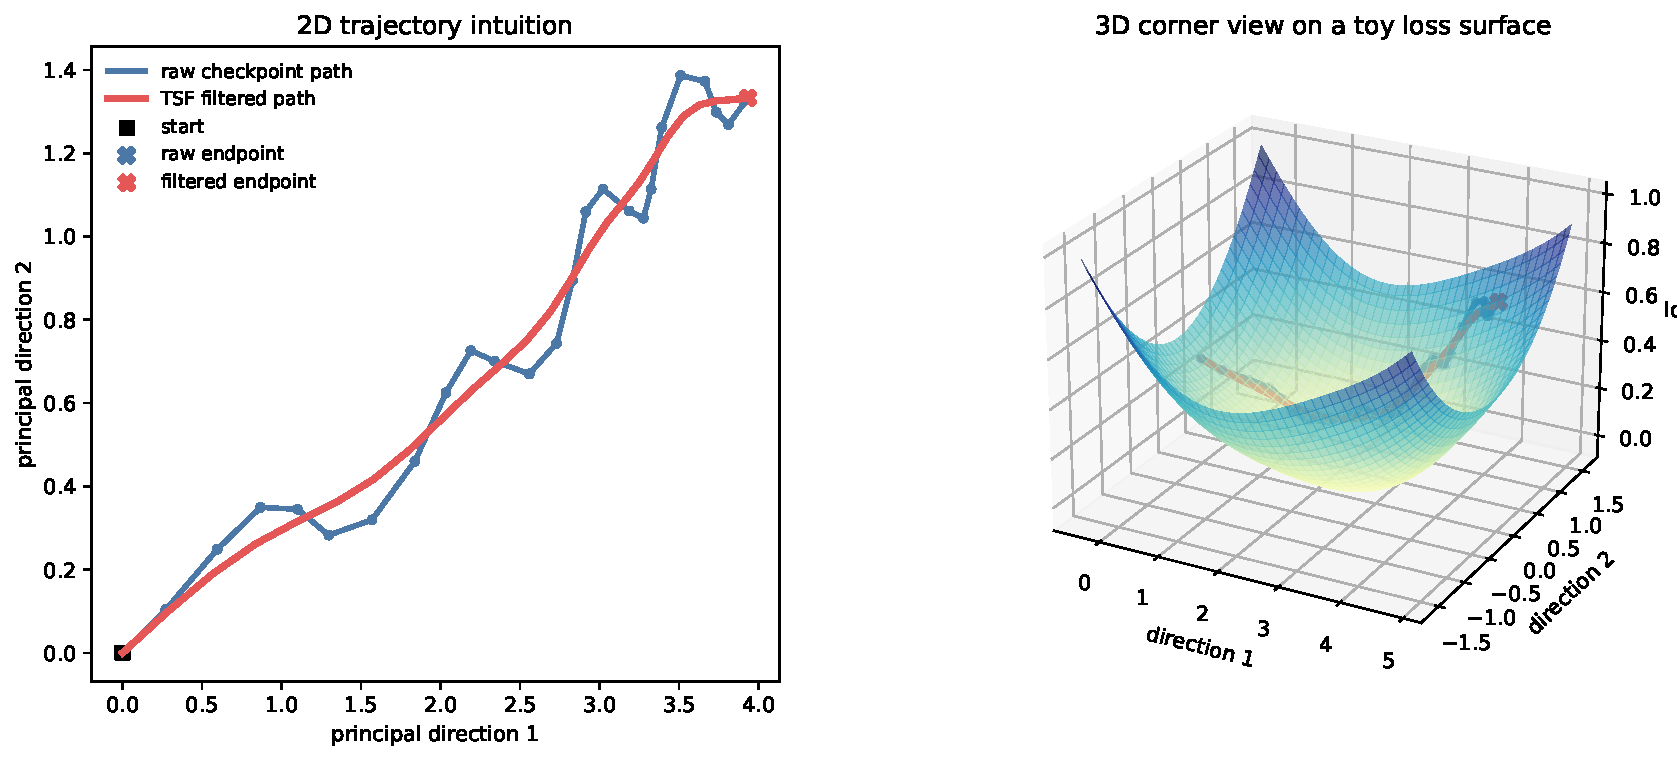
\includegraphics[width=\linewidth]{trajectory_intuition.pdf}
        \caption{2D and 3D intuition.}
        \label{fig:traj_intuition}
    \end{subfigure}
    \hfill
    \begin{subfigure}[t]{0.49\linewidth}
        \centering
        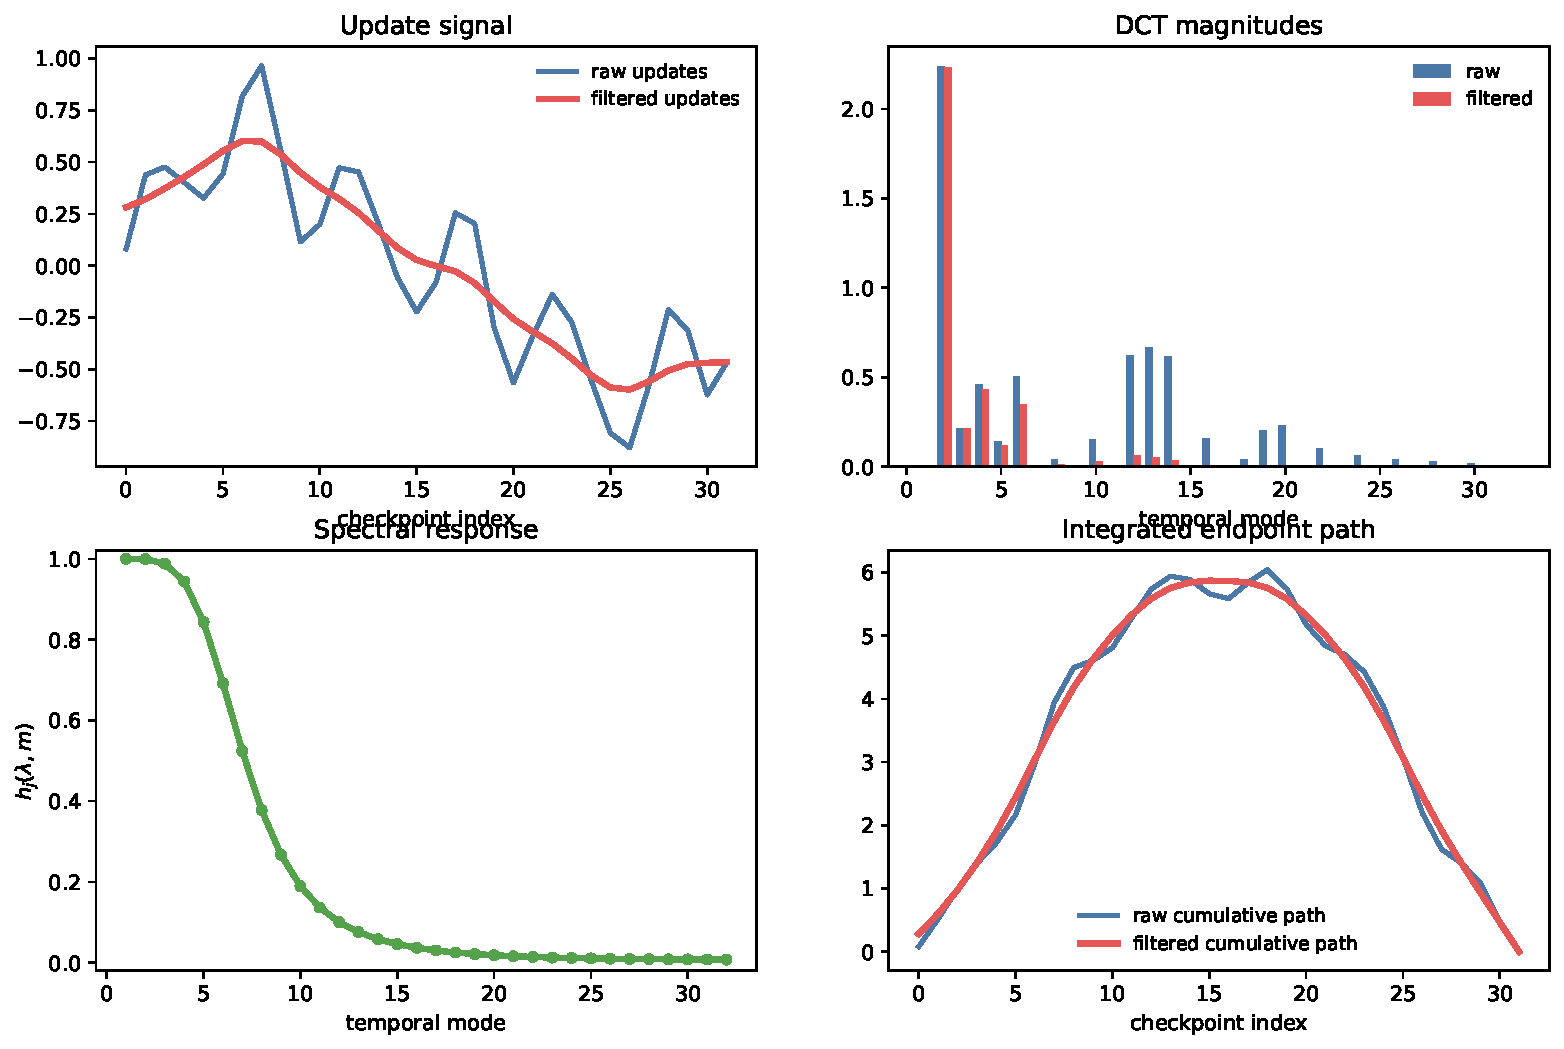
\includegraphics[width=\linewidth]{signal_spectrum.pdf}
        \caption{Signal, spectrum, and filtered path.}
        \label{fig:signal_spectrum}
    \end{subfigure}
    \caption{\textbf{Visual intuition for \tsf{}.} Left: a toy checkpoint path and its filtered counterpart in 2D and on a 3D loss surface viewed from a corner. Right: one update signal, its DCT magnitude profile, the frequency response, and the cumulative filtered path.}
    \label{fig:intuition}
\end{figure}

\begin{algorithm}[t]
\caption{\tsf{}}
\label{alg:tsf}
\begin{algorithmic}[1]
\Require Dense checkpoints \(\theta^{(1)},\ldots,\theta^{(N)}\); grouping \(\cG\); smoothing order \(m\); penalty \(\lambda\)
\State \(n \gets N-1\); construct \(C_n\), \(\Lambda_m\), and \(H_{\lambda,m}\)
\For{each group \(g\in\cG\)}
    \State Extract \(w_g^{(1)},\ldots,w_g^{(N)}\)
    \State Form updates \(v_g^{(t)} = w_g^{(t+1)} - w_g^{(t)}\) for \(t=1,\ldots,n\)
    \State Stack \(V_g \in \RR^{n\times d_g}\)
    \State Compute \(\widetilde V_g = C_n^\top H_{\lambda,m} C_n V_g\)
    \State Reconstruct \(w_g^\star = w_g^{(1)} + \sum_{t=1}^{n} \widetilde v_g^{(t)}\)
\EndFor
\State Assemble \(\theta^\star = \braces{w_g^\star : g\in\cG}\)
\State Optional: refresh batch-normalization statistics once on pooled source data
\State \Return \(\theta^\star\)
\end{algorithmic}
\end{algorithm}

\section{Hidden-Shift Evaluation Functional}
\label{sec:hidden_shift}

To connect \tsf{} to DG, we define a label-free pooled-source hidden-shift evaluation functional. Let
\[
\cU = \braces{(x_i,y_i)}_{i=1}^n
\]
be a pooled labeled source holdout set. For model \(\theta\), define the clipped per-example loss
\begin{equation}
\loss_i(\theta)
=
-\log \max\braces{ p_\theta(x_i)_{y_i}, \varepsilon_p },
\qquad
1\le i\le n,
\label{eq:clipped_loss}
\end{equation}
where \(p_\theta(x)_y\) is the predicted probability of the true class and \(\varepsilon_p\in(0,1)\) is a numerical floor.

Fix \(\alpha \in (0,1]\). The empirical hidden-shift family is the capped simplex
\begin{equation}
\cQ_\alpha^n
=
\braces{
q\in \simplex^n :
q_i \le \frac{1}{\alpha n}
\;\; \forall i }.
\label{eq:capped_simplex}
\end{equation}
Define the empirical hidden-shift risk
\begin{equation}
\widehat R_\alpha(\theta)
=
\max_{q\in\cQ_\alpha^n} \sum_{i=1}^{n} q_i \loss_i(\theta).
\label{eq:hidden_shift_risk}
\end{equation}

\begin{proposition}[Top-\(\alpha\) / empirical-\(\CVaR\) characterization]
\label{prop:topalpha}
Let \(k = \alpha n\) be an integer and let
\[
\loss_{(1)}(\theta)\ge \loss_{(2)}(\theta)\ge \cdots \ge \loss_{(n)}(\theta)
\]
be the support losses sorted in nonincreasing order. Then
\begin{equation}
\widehat R_\alpha(\theta)
=
\frac{1}{k}\sum_{i=1}^{k} \loss_{(i)}(\theta)
=
\Top_\alpha\!\big(\loss_1(\theta),\ldots,\loss_n(\theta)\big).
\label{eq:topalpha}
\end{equation}
For general \(\alpha\), \(\widehat R_\alpha(\theta)\) equals the empirical \(\CVaR_\alpha\) of the loss vector.
\end{proposition}

Proposition~\ref{prop:topalpha} gives an exact adversarial interpretation to the evaluation functional: \(\widehat R_\alpha\) is the average loss on the worst \(\alpha\)-fraction of the pooled support set.

\begin{figure}[t]
    \centering
    \begin{subfigure}[t]{0.49\linewidth}
        \centering
        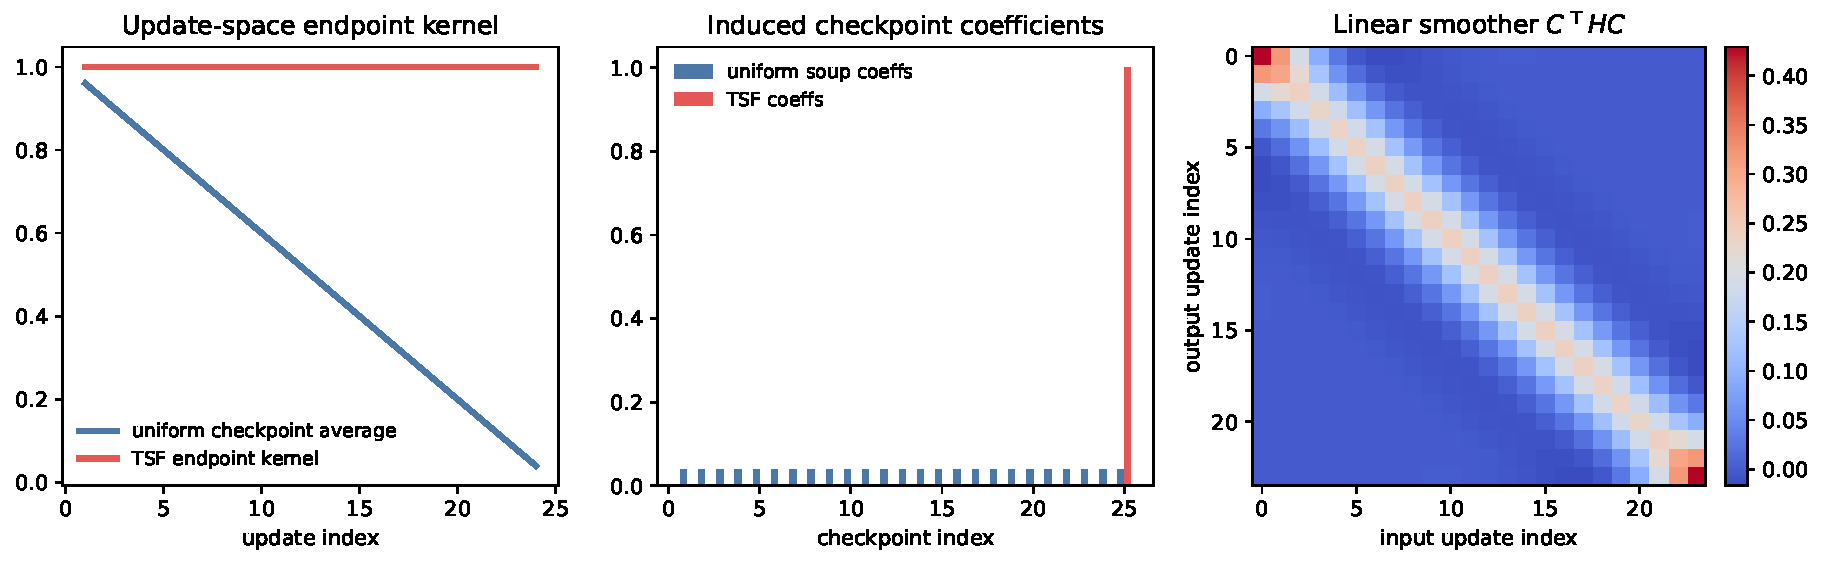
\includegraphics[width=\linewidth]{kernel_comparison.pdf}
        \caption{Uniform averaging vs. \tsf{} kernels.}
        \label{fig:kernels}
    \end{subfigure}
    \hfill
    \begin{subfigure}[t]{0.49\linewidth}
        \centering
        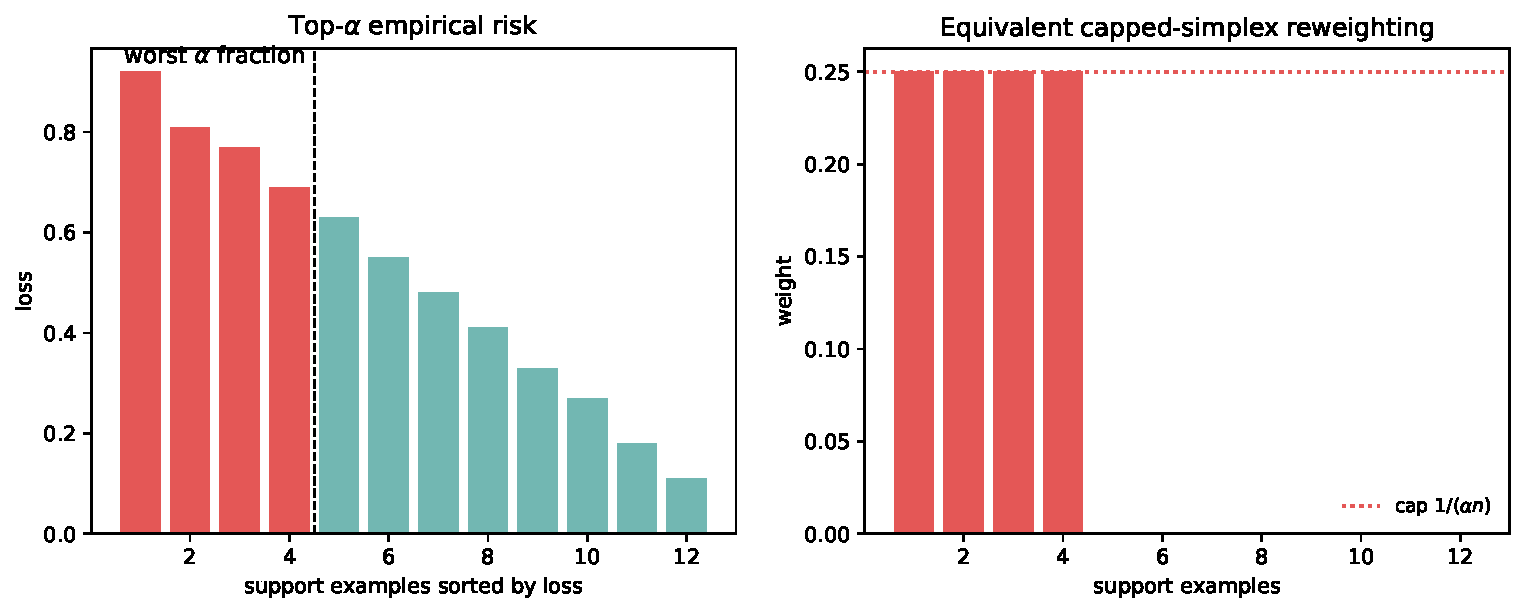
\includegraphics[width=\linewidth]{hidden_shift_topalpha.pdf}
        \caption{Top-\(\alpha\) hidden-shift risk.}
        \label{fig:topalpha}
    \end{subfigure}
    \caption{\textbf{What \tsf{} changes, and how hidden-shift risk is measured.} Left: checkpoint averaging induces a triangular update kernel, while \tsf{} induces a spectrally controlled kernel. Right: the hidden-shift evaluation functional equals the loss on the worst \(\alpha\)-fraction of support examples.}
    \label{fig:kernels_and_topalpha}
\end{figure}

\section{Theoretical Analysis}
\label{sec:theory}

\subsection{Stability and exact bias--variance decomposition}

We first analyze \tsf{} as a denoising operator on the observed update path.

\begin{theorem}[Nonexpansiveness]
\label{thm:nonexpansive}
Fix \(g\in\cG\), \(\lambda\ge 0\), and \(m\in\mathbb{N}\). For any two update matrices \(V_g\) and \(V'_g\),
\begin{equation}
\norm{\widetilde V_g(V_g) - \widetilde V_g(V'_g)}_F
\le
\norm{V_g - V'_g}_F.
\label{eq:nonexp_updates}
\end{equation}
Consequently,
\begin{equation}
\norm{w_g^\star(V_g) - w_g^\star(V'_g)}
\le
\sqrt{n}\,\norm{V_g - V'_g}_F.
\label{eq:nonexp_endpoint}
\end{equation}
\end{theorem}

\begin{assumption}[Groupwise spectral sequence model]
\label{ass:sequence}
For each group \(g\), the observed updates satisfy
\begin{equation}
V_g = S_g + E_g,
\label{eq:signal_model}
\end{equation}
where \(S_g \in \RR^{n\times d_g}\) is a deterministic latent update path and \(E_g\) is zero-mean noise. Writing
\[
\widehat S_g = C_n S_g,
\qquad
\widehat E_g = C_n E_g,
\]
where \(\widehat e_{g,j}\in \RR^{d_g}\) denotes row \(j\) of \(\widehat E_g\).
\end{assumption}

\begin{theorem}[Exact spectral bias--variance decomposition]
\label{thm:bias_variance}
Under Assumption~\ref{ass:sequence},
\begin{equation}
\EE \norm{\widetilde V_g - S_g}_F^2
=
\sum_{j=1}^{n}
\paren{1-h_j(\lambda,m)}^2
\norm{\widehat s_{g,j}}^2
+
\sum_{j=1}^{n}
h_j(\lambda,m)^2\,
\EE \norm{\widehat e_{g,j}}^2,
\label{eq:bias_variance}
\end{equation}
where \(h_j(\lambda,m) = (1+\lambda \rho_j)^{-1}\) and \(\widehat s_{g,j}\) is row \(j\) of \(\widehat S_g\).
\end{theorem}

The first term in Eq.~\eqref{eq:bias_variance} is truncation or smoothing bias; the second is retained variance. This formula is exact, not an inequality.

\begin{corollary}[Strict improvement for sufficiently small positive shrinkage]
\label{cor:strict_improvement}
Fix one group and smoothing order \(m\). Suppose
\begin{equation}
\sum_{j=1}^{n} \rho_j \, \EE\norm{\widehat e_{g,j}}^2 > 0.
\label{eq:strict_improvement_condition}
\end{equation}
Then there exists \(\lambda_0>0\) such that for every \(\lambda\in(0,\lambda_0)\),
\begin{equation}
\EE \norm{\widetilde V_g - S_g}_F^2
<
\EE \norm{V_g - S_g}_F^2
\label{eq:strict_improvement}
\end{equation}
\end{corollary}

\begin{corollary}[Sobolev-type bound]
\label{cor:sobolev}
Assume for one group that
\begin{equation}
\sum_{j=1}^{n} \rho_j \norm{\widehat s_{g,j}}^2 \le R_g^2,
\qquad
\EE\norm{\widehat e_{g,j}}^2 \le \nu_{g,j}.
\label{eq:sobolev_assumption}
\end{equation}
Then
\begin{equation}
\EE \norm{\widetilde V_g - S_g}_F^2
\le
\frac{\lambda R_g^2}{4}
+
\sum_{j=1}^{n} \frac{\nu_{g,j}}{(1+\lambda \rho_j)^2}.
\label{eq:sobolev_bound}
\end{equation}
In particular, if \(\nu_{g,j}\le \bar \nu_g\) for all \(j\), then
\begin{equation}
\EE \norm{\widetilde V_g - S_g}_F^2
\le
\frac{\lambda R_g^2}{4}
+
\bar \nu_g \sum_{j=1}^{n} \frac{1}{(1+\lambda \rho_j)^2}.
\label{eq:sobolev_bound_uniform}
\end{equation}
\end{corollary}

\begin{theorem}[Recovery under vanishing additive noise]
\label{thm:consistency}
Fix a group \(g\), a trajectory length \(n\), and a smoothing order \(m\). Let \(S_g\in\RR^{n\times d_g}\) be a fixed latent update path. Consider a sequence of observations
\[
V_g^{(r)} = S_g + E_g^{(r)},
\qquad r=1,2,\ldots,
\]
and define
\[
\widetilde V_g^{(r)} = C_n^\top H_{\lambda_r,m} C_n V_g^{(r)}.
\]
with
\begin{equation}
\EE \norm{E_g^{(r)}}_F^2 \to 0
\qquad \text{as } r\to\infty.
\label{eq:noise_vanish}
\end{equation}
If \(\lambda_r \to 0\), then
\begin{equation}
\EE \norm{\widetilde V_g^{(r)} - S_g}_F^2 \to 0.
\label{eq:consistency_updates}
\end{equation}
Moreover,
\begin{equation}
\EE \norm{w_{g,r}^\star - w_g^\dagger}^2 \to 0,
\label{eq:endpoint_consistency}
\end{equation}
where
\[
w_g^\dagger = w_g^{(1)} + \sum_{t=1}^{n} s_g^{(t)}.
\]
\end{theorem}

\subsection{From denoising to hidden-shift risk}

We now connect update-path denoising to DG through the hidden-shift functional in Section~\ref{sec:hidden_shift}.

\begin{assumption}[Uniform local smoothness under hidden shifts]
\label{ass:local_smooth}
Let \(\theta^\dagger\) denote the latent reference model obtained by replacing each observed update matrix \(V_g\) by its latent counterpart \(S_g\). Assume there exist constants \(\delta>0\), \(G\ge 0\), and \(\beta\ge 0\) such that for every \(q\in\cQ_\alpha^n\):
\begin{enumerate}[leftmargin=1.4em]
    \item the shifted empirical loss
    \[
    \widehat L_q(\theta)
    =
    \sum_{i=1}^{n} q_i \loss_i(\theta)
    \]
    is differentiable and \(\beta\)-smooth on the ball \(\cB(\theta^\dagger,\delta)\);
    \item the gradient at the reference model is uniformly bounded:
    \[
    \sup_{q\in\cQ_\alpha^n} \norm{\nabla \widehat L_q(\theta^\dagger)} \le G.
    \]
\end{enumerate}
\end{assumption}

\begin{theorem}[Uniform local hidden-shift risk transfer]
\label{thm:risk_transfer}
Under Assumption~\ref{ass:local_smooth}, if \(\norm{\theta^\star - \theta^\dagger}\le \delta\), then
\begin{equation}
\widehat R_\alpha(\theta^\star) - \widehat R_\alpha(\theta^\dagger)
\le
G \norm{\theta^\star - \theta^\dagger}
+
\frac{\beta}{2}\norm{\theta^\star - \theta^\dagger}^2.
\label{eq:risk_transfer}
\end{equation}
If in addition \(\nabla \widehat L_q(\theta^\dagger)=0\) for every \(q\in\cQ_\alpha^n\), then
\begin{equation}
\widehat R_\alpha(\theta^\star) - \widehat R_\alpha(\theta^\dagger)
\le
\frac{\beta}{2}\norm{\theta^\star - \theta^\dagger}^2.
\label{eq:risk_transfer_stationary}
\end{equation}
\end{theorem}

\begin{corollary}[Model-level bound from groupwise path error]
\label{cor:model_level}
Let
\[
\Delta^2 = \sum_{g\in\cG} \norm{\widetilde V_g - S_g}_F^2.
\]
Then
\begin{equation}
\norm{\theta^\star - \theta^\dagger} \le \sqrt{n}\,\Delta.
\label{eq:model_distance}
\end{equation}
Consequently, under Assumption~\ref{ass:local_smooth},
\begin{equation}
\widehat R_\alpha(\theta^\star) - \widehat R_\alpha(\theta^\dagger)
\le
G \sqrt{n}\,\Delta
+
\frac{\beta n}{2}\Delta^2.
\label{eq:combined_bound}
\end{equation}
\end{corollary}

Theorem~\ref{thm:risk_transfer} and Corollary~\ref{cor:model_level} do \emph{not} prove that checkpoint-time high frequencies are ``the'' cause of DG failure. What they do prove is cleaner: if \tsf{} denoises the update path toward a locally good latent reference model, then the worst-case hidden-shift loss moves with that parameter error in a controlled way.

\section{Experimental Protocol and Results Status}
\label{sec:experiments}

\subsection{Protocol}

This paper does not report new \tsf{} numbers yet. The purpose of this section is to make the empirical plan fully explicit and to record exact published context from prior work.

\paragraph{Benchmarks.}
The primary benchmark suite is the standard DomainBed image family \citep{gulrajani2021domainbed}: PACS, VLCS, OfficeHome, TerraIncognita, and DomainNet.

\paragraph{Backbone and training setting.}
The default backbone is ResNet-50, following the reporting style in \swad{} and related papers. Training uses standard \erm{} with dense checkpointing. Post-hoc methods are evaluated on the same saved trajectory.

\paragraph{Baselines.}
At minimum, \tsf{} should be compared against:
\begin{itemize}[leftmargin=1.4em]
    \item final checkpoint,
    \item checkpoint EMA,
    \item moving average over updates,
    \item uniform late-window averaging,
    \item \swad{},
    \item and any stronger published single-model DG baseline reported under the same backbone.
\end{itemize}

\paragraph{Primary \tsf{} ablations.}
The core ablations are:
\begin{itemize}[leftmargin=1.4em]
    \item update filtering vs. absolute-weight filtering,
    \item full trajectory vs. late subsequence,
    \item groupwise vs. scalar filtering,
    \item smoothing order \(m\),
    \item penalty strength \(\lambda\),
    \item with and without batch-normalization refresh,
    \item sensitivity to checkpoint density.
\end{itemize}

\paragraph{Diagnostics.}
The experimental logs should include:
\begin{itemize}[leftmargin=1.4em]
    \item spectral energy retained per group,
    \item model distance to the raw endpoint,
    \item model distance to simple smoothing baselines,
    \item hidden-shift tail risk on pooled support data,
    \item and the induced checkpoint coefficients from Proposition~\ref{prop:endpoint_repr}.
\end{itemize}

\subsection{Published benchmark context}

Table~\ref{tab:published_context} records exact published numbers from prior work. These are not \tsf{} results; they define the current bar.

\begin{table}[t]
    \centering
    \small
    \caption{\textbf{Published DomainBed context from prior work.} The upper block reproduces the single-number reporting style of \citet{cha2021swad}; the lower block uses the ResNet-50 comparison rows reproduced in \citet{teterwak2025ermpp}.}
    \label{tab:published_context}
    \setlength{\tabcolsep}{5pt}
    \begin{tabular}{lcccccc}
        \toprule
        Method & PACS & VLCS & OfficeHome & TerraInc. & DomainNet & Avg. \\
        \midrule
        \erm{} \citep{cha2021swad} & 85.5 & 77.5 & 66.5 & 46.1 & 40.9 & 63.3 \\
        \swad{} \citep{cha2021swad} & 88.1 & 79.1 & 70.6 & 50.0 & 46.5 & 66.9 \\
        \midrule
        \miro{} \citep{teterwak2025ermpp} & \(85.4\pm0.4\) & \(79.0\pm0.0\) & \(70.5\pm0.4\) & \(50.4\pm1.1\) & \(44.3\pm0.2\) & 65.9 \\
        \miro{}+\swad{} \citep{teterwak2025ermpp} & \(88.4\pm0.1\) & \(79.6\pm0.2\) & \(72.4\pm0.1\) & \(52.9\pm0.2\) & \(47.0\pm0.0\) & 68.1 \\
        \bottomrule
    \end{tabular}
\end{table}

\begin{table}[t]
    \centering
    \small
    \caption{\textbf{Published average-only context from stronger or different settings.} These rows are useful frontier markers, but not all are identical to the plain single-run post-hoc setting targeted by \tsf{}.}
    \label{tab:published_context_avg}
    \begin{tabular}{lll}
        \toprule
        Setting & Method & Avg. \\
        \midrule
        Published post-hoc DG & \eoa{} \citep{arpit2022eoa} & 68.0 \\
        Hybrid post-hoc DG & \miro{}+\swad{} \citep{teterwak2025ermpp} & 68.1 \\
        Stronger training baseline & \ermpp{} \citep{teterwak2025ermpp} & 68.9 \\
        \bottomrule
    \end{tabular}
\end{table}

\subsection{\tsf{} reporting templates}

\begin{table}[t]
    \centering
    \small
    \caption{\textbf{Primary \tsf{} reporting table.}}
    \label{tab:tsf_main}
    \setlength{\tabcolsep}{6pt}
    \begin{tabular}{lcccccc}
        \toprule
        Method & PACS & VLCS & OfficeHome & TerraInc. & DomainNet & Avg. \\
        \midrule
        \tsf{} & \TBD & \TBD & \TBD & \TBD & \TBD & \TBD \\
        \tsf{} + BN refresh & \TBD & \TBD & \TBD & \TBD & \TBD & \TBD \\
        \tsf{} + stronger backbone & \TBD & \TBD & \TBD & \TBD & \TBD & \TBD \\
        \bottomrule
    \end{tabular}
\end{table}

\begin{table}[t]
    \centering
    \small
    \caption{\textbf{\tsf{} ablation table.}}
    \label{tab:tsf_ablation}
    \setlength{\tabcolsep}{7pt}
    \begin{tabular}{lccc}
        \toprule
        Variant & PACS & Avg. & Comment \\
        \midrule
        \tsf{} baseline & \TBD & \TBD & full trajectory, groupwise, update filtering \\
        Late subsequence only & \TBD & \TBD & full vs. late trajectory \\
        EMA baseline & \TBD & \TBD & nearest smoothing baseline \\
        Moving-average updates & \TBD & \TBD & nearest smoothing baseline \\
        Weight filtering instead of updates & \TBD & \TBD & object ablation \\
        Scalar filtering instead of groups & \TBD & \TBD & grouping ablation \\
        \bottomrule
    \end{tabular}
\end{table}

\begin{table}[t]
    \centering
    \small
    \caption{\textbf{Core \tsf{} diagnostics.}}
    \label{tab:tsf_diagnostics}
    \begin{tabular}{lcc}
        \toprule
        Diagnostic & Value & Status \\
        \midrule
        Retained spectral energy fraction & \TBD & \TBD \\
        Distance to raw endpoint & \TBD & \TBD \\
        Distance to EMA baseline & \TBD & \TBD \\
        Hidden-shift tail risk on support split & \TBD & \TBD \\
        Checkpoint-density sensitivity & \TBD & \TBD \\
        \bottomrule
    \end{tabular}
\end{table}

\section{Discussion and Limitations}
\label{sec:discussion}

\tsf{} is intentionally more cautious than the strongest possible story one might tell about checkpoint trajectories.

\paragraph{What the theory does establish.}
The theory establishes that:
\begin{itemize}[leftmargin=1.4em]
    \item the main filter family is the exact solution of a convex smoothing problem,
    \item the operator is stable,
    \item the denoising error admits an exact spectral bias--variance decomposition,
    \item and local hidden-shift loss moves with parameter error.
\end{itemize}

\paragraph{What the theory does \emph{not} establish.}
The theory does \emph{not} establish that:
\begin{itemize}[leftmargin=1.4em]
    \item checkpoint-time high frequency always equals harmful fitting,
    \item low checkpoint-time frequency always equals robust/invariant structure,
    \item or full-trajectory filtering is always better than local late-window smoothing.
\end{itemize}

\paragraph{Why this still counts as a DG method.}
The method is aimed at DG because it produces one deployment model using only source data and is evaluated under hidden-shift tail risk. But the theory is deliberately layered:
\begin{itemize}[leftmargin=1.4em]
    \item first, a denoising theorem on the update path;
    \item second, a local hidden-shift risk transfer theorem.
\end{itemize}
This is more defensible than claiming that checkpoint-frequency filtering directly solves DG.

\paragraph{The most dangerous alternative explanation.}
The strongest null hypothesis is that \tsf{} is just a more complicated linear smoother. The paper therefore treats checkpoint EMA and moving-average update smoothing as first-class baselines, not afterthoughts.

\paragraph{Full trajectory vs. late locality.}
The main paper studies the full trajectory because that is the distinctive hypothesis. If the only successful variant ends up using a late local window and behaves like ordinary smoothing, then \tsf{} no longer supports a strong methodological claim. The planned experiments are designed to decide that directly.

\section{Conclusion}

This paper proposes \tsf{}, a post-hoc DG method that smooths the groupwise checkpoint update path rather than selecting or averaging checkpoints directly. The method is mathematically concrete: its main filter family is the unique solution of a spectral Sobolev-type smoothing problem. The paper then proves exact operator identities, denoising guarantees, and a conditional local hidden-shift risk bound. What remains open is empirical. If \tsf{} cannot beat simple smoothing baselines, then the right conclusion is that spectral filtering of checkpoint updates does not unlock enough new structure beyond existing averaging methods. If it can, then it identifies a genuinely different post-hoc operator inside the checkpoint-trajectory regime.

\section*{Acknowledgments}

This section is intentionally omitted for anonymous review.

\bibliographystyle{plainnat}
\bibliography{references}

\appendix

\section{Additional Visual Intuition}

\begin{figure}[H]
    \centering
    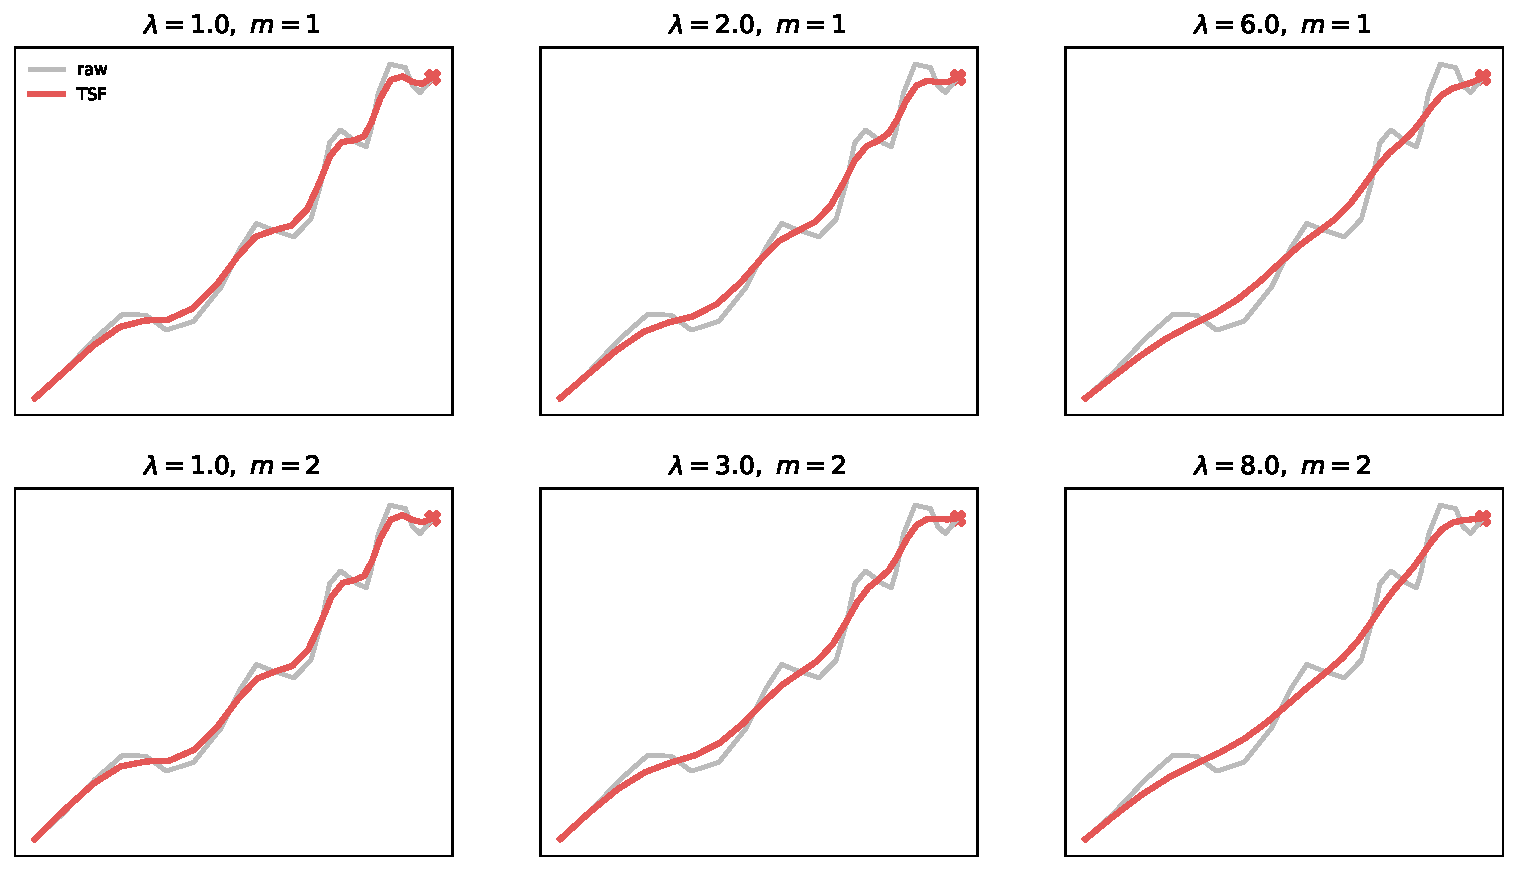
\includegraphics[width=0.9\linewidth]{filter_family_grid.pdf}
    \caption{\textbf{Filter-family intuition.} Different values of \(\lambda\) and smoothing order \(m\) produce different filtered paths on the same toy update sequence. Larger \(\lambda\) and higher \(m\) remove more temporal roughness.}
    \label{fig:filter_grid}
\end{figure}

\section{Proofs}

\subsection{Proof of Proposition~\ref{prop:variational}}

\begin{proof}
Let \(\widehat U = C_n U\) and \(\widehat V_g = C_n V_g\). Since \(C_n\) is orthonormal,
\[
\norm{U - V_g}_F^2 = \norm{\widehat U - \widehat V_g}_F^2.
\]
Likewise,
\[
\norm{\Lambda_m^{1/2} C_n U}_F^2 = \norm{\Lambda_m^{1/2} \widehat U}_F^2.
\]
Therefore the objective in Eq.~\eqref{eq:variational} becomes
\[
\frac12 \norm{\widehat U - \widehat V_g}_F^2
+
\frac{\lambda}{2}\norm{\Lambda_m^{1/2}\widehat U}_F^2.
\]
Write \(\widehat U\) row-wise as \(\widehat u_1,\ldots,\widehat u_n\in\RR^{d_g}\), and similarly \(\widehat v_1,\ldots,\widehat v_n\). The objective decomposes as
\[
\sum_{j=1}^{n}
\left[
\frac12 \norm{\widehat u_j - \widehat v_j}^2
+
\frac{\lambda \rho_j}{2}\norm{\widehat u_j}^2
\right].
\]
Each summand is strictly convex in \(\widehat u_j\), so the minimizer is unique and can be found by differentiating:
\[
0 = \widehat u_j - \widehat v_j + \lambda \rho_j \widehat u_j
=
(1+\lambda \rho_j)\widehat u_j - \widehat v_j.
\]
Hence
\[
\widehat u_j = \frac{1}{1+\lambda \rho_j}\widehat v_j = h_j(\lambda,m)\widehat v_j.
\]
Stacking the rows yields
\[
\widehat U = H_{\lambda,m} \widehat V_g.
\]
Multiplying by \(C_n^\top\) gives
\[
U = C_n^\top H_{\lambda,m} C_n V_g = \widetilde V_g(\lambda,m).
\]
This proves Eq.~\eqref{eq:tsf_updates}.

For Eq.~\eqref{eq:variational_q}, note that
\[
\norm{\Lambda_m^{1/2} C_n U}_F^2
=
\tr\!\left( U^\top C_n^\top \Lambda_m C_n U \right)
=
\inner{U}{Q_m U}_F,
\]
where \(Q_m = C_n^\top \Lambda_m C_n\). The minimizer is the same. The strong convexity of the quadratic objective implies uniqueness.
\end{proof}

\subsection{Proof of Proposition~\ref{prop:endpoint_repr}}

\begin{proof}
By definition,
\[
w^\star = w^{(1)} + \sum_{t=1}^{n} \widetilde v^{(t)}.
\]
Since \(\widetilde V = C_n^\top H_{\lambda,m} C_n V\), the sum of filtered updates is
\[
\sum_{t=1}^{n} \widetilde v^{(t)}
=
\mathbf{1}^\top \widetilde V
=
\mathbf{1}^\top C_n^\top H_{\lambda,m} C_n V
=
a^\top V
=
\sum_{t=1}^{n} a_t v^{(t)},
\]
which proves the first identity in Eq.~\eqref{eq:checkpoint_coeffs}.

Now use
\[
v^{(t)} = w^{(t+1)} - w^{(t)}.
\]
Then
\begin{align*}
w^\star
&=
w^{(1)} + \sum_{t=1}^{n} a_t \paren{w^{(t+1)} - w^{(t)}} \\
&=
\paren{1-a_1} w^{(1)}
+
\sum_{t=2}^{n} \paren{a_{t-1}-a_t} w^{(t)}
+
a_n w^{(n+1)}.
\end{align*}
This is Eq.~\eqref{eq:alpha_formula}.

Finally, for the uniform checkpoint average,
\[
\bar w = \frac{1}{n+1}\sum_{s=1}^{n+1} w^{(s)}.
\]
Using
\[
w^{(s)} = w^{(1)} + \sum_{t=1}^{s-1} v^{(t)},
\]
we obtain
\begin{align*}
\bar w
&=
\frac{1}{n+1}\sum_{s=1}^{n+1}
\paren{
w^{(1)} + \sum_{t=1}^{s-1} v^{(t)}
} \\
&=
w^{(1)}
+
\frac{1}{n+1}
\sum_{t=1}^{n}
\sum_{s=t+1}^{n+1} v^{(t)} \\
&=
w^{(1)}
+
\sum_{t=1}^{n}
\frac{n+1-t}{n+1}
v^{(t)}.
\end{align*}
This proves Eq.~\eqref{eq:uniform_update_kernel}.
\end{proof}

\subsection{Proof of Proposition~\ref{prop:topalpha}}

\begin{proof}
We first assume \(k=\alpha n\) is an integer. The feasible region
\[
\cQ_\alpha^n
=
\braces{
q\in\RR^n :
q_i\ge 0,\;
\sum_{i=1}^{n} q_i = 1,\;
q_i \le 1/k
}
\]
is a compact polytope, so the linear objective
\[
q \mapsto \sum_{i=1}^{n} q_i \loss_i(\theta)
\]
attains its maximum at an extreme point.

Every extreme point of \(\cQ_\alpha^n\) has exactly \(k\) entries equal to \(1/k\) and the rest equal to \(0\). Indeed, if an extreme point had fewer than \(k\) positive coordinates, then because each positive coordinate is at most \(1/k\), the sum could not equal \(1\). If it had more than \(k\) positive coordinates, then at least two of them would lie strictly between \(0\) and \(1/k\), and one could perturb mass between those two coordinates while staying feasible, contradicting extremality.

Therefore maximizing over \(\cQ_\alpha^n\) is equivalent to choosing a subset of \(k\) examples and assigning each chosen example weight \(1/k\). The maximizing subset is the one containing the \(k\) largest losses. Hence
\[
\widehat R_\alpha(\theta)
=
\frac{1}{k}\sum_{i=1}^{k} \loss_{(i)}(\theta).
\]
This is exactly the top-\(\alpha\) empirical mean.

For general \(\alpha\), the feasible polytope has the same form except that \(1/(\alpha n)\) need not correspond to an integer support size. The maximization is then the empirical \(\CVaR_\alpha\) of the loss vector, equivalently the standard top-\(\alpha\) mean with fractional interpolation at the boundary. This is the finite-dimensional linear-programming representation of empirical \(\CVaR\).
\end{proof}

\subsection{Proof of Theorem~\ref{thm:nonexpansive}}

\begin{proof}
Let \(T_{\lambda,m}=C_n^\top H_{\lambda,m} C_n\). Since \(C_n\) is orthonormal and \(H_{\lambda,m}\) is diagonal with entries in \([0,1]\),
\[
\norm{T_{\lambda,m}}_{\mathrm{op}}
=
\norm{H_{\lambda,m}}_{\mathrm{op}}
=
\max_j h_j(\lambda,m)
\le
1.
\]
Therefore
\[
\norm{T_{\lambda,m}(V_g - V'_g)}_F
\le
\norm{V_g - V'_g}_F.
\]
But \(T_{\lambda,m}(V_g)=\widetilde V_g(V_g)\), so Eq.~\eqref{eq:nonexp_updates} follows.

For the endpoint bound,
\[
w_g^\star(V_g) - w_g^\star(V'_g)
=
\sum_{t=1}^{n}\paren{\widetilde v_g^{(t)}(V_g) - \widetilde v_g^{(t)}(V'_g)}.
\]
Applying Cauchy--Schwarz gives
\[
\norm{w_g^\star(V_g) - w_g^\star(V'_g)}
\le
\sqrt{n}
\left(
\sum_{t=1}^{n}
\norm{\widetilde v_g^{(t)}(V_g) - \widetilde v_g^{(t)}(V'_g)}^2
\right)^{1/2}
=
\sqrt{n}\,\norm{\widetilde V_g(V_g) - \widetilde V_g(V'_g)}_F.
\]
Combine this with Eq.~\eqref{eq:nonexp_updates} to obtain Eq.~\eqref{eq:nonexp_endpoint}.
\end{proof}

\subsection{Proof of Theorem~\ref{thm:bias_variance}}

\begin{proof}
Write
\[
\widehat V_g = C_n V_g = \widehat S_g + \widehat E_g.
\]
The filtered estimator in the spectral domain is
\[
\widehat{\widetilde V}_g
=
H_{\lambda,m}\widehat V_g.
\]
Therefore
\[
\widehat{\widetilde V}_g - \widehat S_g
=
(H_{\lambda,m}-I)\widehat S_g + H_{\lambda,m}\widehat E_g.
\]
Because \(C_n\) is orthonormal,
\[
\norm{\widetilde V_g - S_g}_F
=
\norm{\widehat{\widetilde V}_g - \widehat S_g}_F.
\]
Taking squared Frobenius norms and expectations yields
\begin{align*}
\EE\norm{\widetilde V_g - S_g}_F^2
&=
\EE\norm{(H_{\lambda,m}-I)\widehat S_g + H_{\lambda,m}\widehat E_g}_F^2 \\
&=
\norm{(H_{\lambda,m}-I)\widehat S_g}_F^2
+
\EE\norm{H_{\lambda,m}\widehat E_g}_F^2 \\
&\qquad
+
2\,\EE\inner{(H_{\lambda,m}-I)\widehat S_g}{H_{\lambda,m}\widehat E_g}_F.
\end{align*}
The cross term is zero because \(\EE[\widehat E_g]=0\). Expanding row-wise,
\[
\norm{(H_{\lambda,m}-I)\widehat S_g}_F^2
=
\sum_{j=1}^{n}
(1-h_j)^2 \norm{\widehat s_{g,j}}^2.
\]
Likewise,
\[
\EE\norm{H_{\lambda,m}\widehat E_g}_F^2
=
\sum_{j=1}^{n} h_j^2 \EE\norm{\widehat e_{g,j}}^2,
\]
because the Frobenius norm is the sum of squared row norms. This proves Eq.~\eqref{eq:bias_variance}.
\end{proof}

\subsection{Proof of Corollary~\ref{cor:strict_improvement}}

\begin{proof}
Define
\[
M(\lambda)
=
\EE \norm{\widetilde V_g(\lambda,m) - S_g}_F^2.
\]
At \(\lambda=0\), the filter is the identity, so
\[
M(0)
=
\EE\norm{V_g - S_g}_F^2
=
\sum_{j=1}^{n}\EE\norm{\widehat e_{g,j}}^2,
\]
because \(V_g-S_g = E_g\) and \(C_n\) is orthonormal.

By Theorem~\ref{thm:bias_variance},
\[
M(\lambda)-M(0)
=
\sum_{j=1}^{n}
\left[
(1-h_j)^2 \norm{\widehat s_{g,j}}^2
-
(1-h_j^2)\EE\norm{\widehat e_{g,j}}^2
\right].
\]
Using \(h_j(\lambda,m)=(1+\lambda \rho_j)^{-1}\), we obtain
\[
\frac{M(\lambda)-M(0)}{\lambda}
=
\sum_{j=1}^{n}
\frac{
\lambda \rho_j^2 \norm{\widehat s_{g,j}}^2
-
(2\rho_j+\lambda \rho_j^2)\EE\norm{\widehat e_{g,j}}^2
}{
(1+\lambda \rho_j)^2
}.
\]
For each \(j\), the summand converges as \(\lambda\downarrow 0\) to
\[
-2\rho_j \EE\norm{\widehat e_{g,j}}^2.
\]
Therefore
\[
\lim_{\lambda\downarrow 0}
\frac{M(\lambda)-M(0)}{\lambda}
=
-2\sum_{j=1}^{n}\rho_j \EE\norm{\widehat e_{g,j}}^2
<
0
\]
by Eq.~\eqref{eq:strict_improvement_condition}. By continuity of \(M\), there exists \(\lambda_0>0\) such that
\[
M(\lambda) < M(0)
\qquad \text{for all } \lambda\in(0,\lambda_0).
\]
This is Eq.~\eqref{eq:strict_improvement}.
\end{proof}

\subsection{Proof of Corollary~\ref{cor:sobolev}}

\begin{proof}
By Theorem~\ref{thm:bias_variance},
\[
\EE \norm{\widetilde V_g - S_g}_F^2
=
\sum_{j=1}^{n}(1-h_j)^2\norm{\widehat s_{g,j}}^2
+
\sum_{j=1}^{n} h_j^2 \EE\norm{\widehat e_{g,j}}^2.
\]
For the variance term, use the bound \(\EE\norm{\widehat e_{g,j}}^2 \le \nu_{g,j}\).

For the bias term, let \(x_j=\lambda \rho_j\). Since \(h_j=(1+x_j)^{-1}\),
\[
(1-h_j)^2
=
\left( \frac{x_j}{1+x_j} \right)^2.
\]
For \(x\ge 0\),
\[
\frac{x^2}{(1+x)^2}
=
x \cdot \frac{x}{(1+x)^2}
\le
\frac{x}{4},
\]
because \(x/(1+x)^2 \le 1/4\) for all \(x\ge 0\), with equality at \(x=1\). Therefore
\[
(1-h_j)^2 \le \frac{\lambda \rho_j}{4}.
\]
Hence
\[
\sum_{j=1}^{n}(1-h_j)^2\norm{\widehat s_{g,j}}^2
\le
\frac{\lambda}{4}
\sum_{j=1}^{n}\rho_j \norm{\widehat s_{g,j}}^2
\le
\frac{\lambda R_g^2}{4}.
\]
This proves Eq.~\eqref{eq:sobolev_bound}. The uniform-noise version follows by replacing each \(\nu_{g,j}\) by \(\bar\nu_g\).
\end{proof}

\subsection{Proof of Theorem~\ref{thm:consistency}}

\begin{proof}
Let \(T_r = C_n^\top H_{\lambda_r,m} C_n\). Then
\[
\widetilde V_g^{(r)} - S_g
=
T_r(S_g + E_g^{(r)}) - S_g
=
T_r E_g^{(r)} + (T_r-I)S_g.
\]
Using \(\norm{A+B}_F^2 \le 2\norm{A}_F^2 + 2\norm{B}_F^2\),
\[
\EE \norm{\widetilde V_g^{(r)} - S_g}_F^2
\le
2\,\EE \norm{T_r E_g^{(r)}}_F^2
+
2\,\norm{(T_r-I)S_g}_F^2.
\]
By Theorem~\ref{thm:nonexpansive},
\[
\EE \norm{T_r E_g^{(r)}}_F^2
\le
\EE \norm{E_g^{(r)}}_F^2.
\]
Also,
\[
\norm{(T_r-I)S_g}_F
\le
\norm{T_r-I}_{\mathrm{op}} \norm{S_g}_F.
\]
Since \(T_r\) is orthogonally diagonalized by \(C_n\),
\[
\norm{T_r-I}_{\mathrm{op}}
=
\max_{1\le j\le n} \abs{h_j(\lambda_r,m)-1}.
\]
For every \(j\), \(h_j(\lambda_r,m)=(1+\lambda_r\rho_j)^{-1}\to 1\) as \(r\to\infty\), so \(\norm{T_r-I}_{\mathrm{op}}\to 0\). Together with Eq.~\eqref{eq:noise_vanish}, this proves Eq.~\eqref{eq:consistency_updates}.

For the endpoint claim,
\[
w_{g,r}^\star - w_g^\dagger
=
\sum_{t=1}^{n}\paren{\widetilde v_g^{(t,r)} - s_g^{(t)}}.
\]
By Cauchy--Schwarz,
\[
\norm{w_{g,r}^\star - w_g^\dagger}^2
\le
n
\sum_{t=1}^{n}\norm{\widetilde v_g^{(t,r)} - s_g^{(t)}}^2
=
n \norm{\widetilde V_g^{(r)} - S_g}_F^2.
\]
Taking expectations and using Eq.~\eqref{eq:consistency_updates} yields Eq.~\eqref{eq:endpoint_consistency}.
\end{proof}

\subsection{Proof of Theorem~\ref{thm:risk_transfer}}

\begin{proof}
Fix \(q\in\cQ_\alpha^n\). Since \(\widehat L_q\) is \(\beta\)-smooth on \(\cB(\theta^\dagger,\delta)\), the standard descent lemma gives, for any \(\theta\in\cB(\theta^\dagger,\delta)\),
\[
\widehat L_q(\theta)
\le
\widehat L_q(\theta^\dagger)
+
\inner{\nabla \widehat L_q(\theta^\dagger)}{\theta-\theta^\dagger}
+
\frac{\beta}{2}\norm{\theta-\theta^\dagger}^2.
\]
Apply this at \(\theta=\theta^\star\). Using Cauchy--Schwarz and the uniform gradient bound,
\[
\widehat L_q(\theta^\star) - \widehat L_q(\theta^\dagger)
\le
\norm{\nabla \widehat L_q(\theta^\dagger)}\,\norm{\theta^\star-\theta^\dagger}
+
\frac{\beta}{2}\norm{\theta^\star-\theta^\dagger}^2
\le
G\norm{\theta^\star-\theta^\dagger}
+
\frac{\beta}{2}\norm{\theta^\star-\theta^\dagger}^2.
\]
This holds for every \(q\in\cQ_\alpha^n\). Taking the supremum over \(q\) and using the definition of \(\widehat R_\alpha\) from Eq.~\eqref{eq:hidden_shift_risk} yields Eq.~\eqref{eq:risk_transfer}.

If \(\nabla \widehat L_q(\theta^\dagger)=0\) for every \(q\), then the linear term vanishes and Eq.~\eqref{eq:risk_transfer_stationary} follows.
\end{proof}

\subsection{Proof of Corollary~\ref{cor:model_level}}

\begin{proof}
For each group,
\[
w_g^\star - w_g^\dagger
=
\sum_{t=1}^{n}\paren{\widetilde v_g^{(t)} - s_g^{(t)}}.
\]
By Cauchy--Schwarz,
\[
\norm{w_g^\star - w_g^\dagger}^2
\le
n \norm{\widetilde V_g - S_g}_F^2.
\]
Summing over groups gives
\[
\norm{\theta^\star - \theta^\dagger}^2
=
\sum_{g\in\cG}\norm{w_g^\star - w_g^\dagger}^2
\le
n \sum_{g\in\cG}\norm{\widetilde V_g - S_g}_F^2
=
n \Delta^2.
\]
Taking square roots proves Eq.~\eqref{eq:model_distance}. Plug Eq.~\eqref{eq:model_distance} into Theorem~\ref{thm:risk_transfer} to obtain Eq.~\eqref{eq:combined_bound}.
\end{proof}

\section{Additional Experimental Templates}

\begin{table}[H]
    \centering
    \small
    \caption{\textbf{Planned checkpoint-density sensitivity table.}}
    \label{tab:density_tbd}
    \begin{tabular}{lccc}
        \toprule
        Checkpoint stride & PACS & Avg. & Comment \\
        \midrule
        Full density & \TBD & \TBD & default replay bank \\
        Every 2nd checkpoint & \TBD & \TBD & subsampling test \\
        Every 4th checkpoint & \TBD & \TBD & subsampling test \\
        \bottomrule
    \end{tabular}
\end{table}

\end{document}
